%\setcounter{framenumber}{30}
\makeatletter
\ifodd\value{page}
\else
\begin{frame}[plain]
\end{frame}
\fi
\makeatother


\section{张量简介*}


\title{第十章 \quad 张量简介*}
\author{}
\date{}

\frame{\titlepage}

\subsection{引言(张量)*}

\subsubsection{张量简介*}
\begin{frame}\frametitle{张量简介*}
在物理学中, 张量的任务是描述物理量坐标变换时的变换规律。其提供了一个简明的数学框架用来描述和解决力学（应力、弹性、流体力学、惯性矩等）、电动力学（电磁张量、麦克斯韦张量、介电常数、磁化率等）、广义相对论（应力-能量张量、曲率张量等）物理问题。

\pp
\bigskip

有两种定义张量的方法:\pp
\begin{enumerate}
\item 通常定义张量的物理学或传统数学方法,是把张量看成一个多维数组,当变换坐标或变换基底时,其分量会按照一定的规则变换.\pp
\item 现代数学中的方法,是把张量定义成某个向量空间或其对偶空间上的多重线性映射,这向量空间在需要引入基底之前不固定任何坐标系统。
\end{enumerate}\pp

\bigskip
经典物理学中将一阶张量归结为向量(矢量)、二阶张量归结为并矢．但到了相对论力学、电动力学和引力理论中,空间成为非欧氏的,甚至是弯曲的,这时就不可避免地需要运用张量分析.
\end{frame}




\subsubsection{物理学中的张量--应力张量(stress tensor)*}
\begin{frame}\frametitle{物理学中的张量--应力张量(stress tensor)*}
应力张量是描述物体内部应力分布的重要工具.
\pp

下面我们看P处的应力张量:
\begin{center}
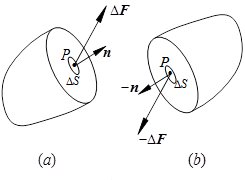
\includegraphics[width=0.3\linewidth]{pic/2013-07-30-01}
\end{center}

\pp
\begin{center}
 面积元 $\Delta S$  $\xmapsto[\text{应力张量}]{\text{$P$处应力分布}}$ 作用力 $\Delta F$.
\end{center}

\pp
若将面积元和作用力视为空间向量,则应力张量为三维空间的一个\blue{线性变换}.
\pp

通过选定三维空间的一个(直角)坐标系,则应力张量可表示为一个$3$阶方阵.
\begin{center}
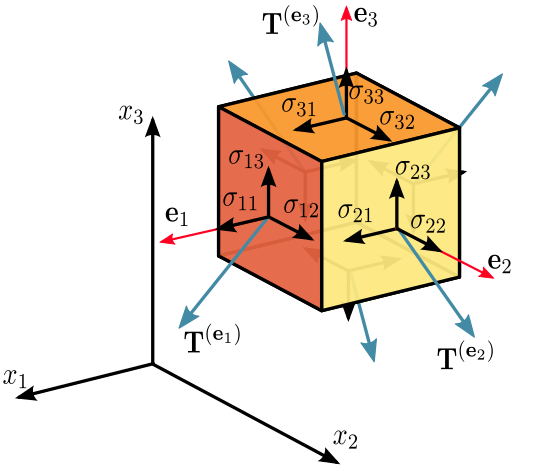
\includegraphics[width=0.2\linewidth]{pic/Components_stress_tensor}
\end{center}
\end{frame}



\subsection{本课程中的张量*}

\subsubsection{线性代数(B1)课程中学到的张量*}
\begin{frame}\frametitle{线性代数(B1)课程中学到的张量*}
给定域$\bF$上的一个线性空间$V$. 设$P$为从基$e=(e_1,\cdots,e_n)$到基$e'=(e'_1,\cdots,e'_n)$的过渡矩阵.
\pp
即
\[(e'_1,\cdots,e'_n)=(e_1,\cdots,e_n)P \qquad \text{或}\qquad  \blue{e'_j = \sum_{i=1}^{n} e_i \cdot (P)^i_j}.\]
其中任意矩阵$A$,记$(A)^i_j$为$A$的第$i$行$j$列的元素. 对于任意列向量$X$,记$(X)^i$为$X$的第$i$个元素.
\pp

\bigskip
\begin{enumerate}
\item 线性空间$V$中的向量;  	\hfill{($(1,0)$-型张量)}
\pp
\begin{center}
$V$中向量 $\xrightarrow[v=(e_1,\cdots,e_n)X]{\text{$V$的一组基}}$   坐标 + 坐标变换公式(逆变)
\end{center}
\pp
\[X' = P^{-1}X \qquad \text{或}\qquad  \blue{(X')^i = \sum_{j=1}^{n} (X)^j\cdot (P^{-1})^i_j}\]
\pp

\item 线性空间$V$上的线性变换; \hfill{($(1,1)$-型张量)}
\pp
\begin{center}
线性变换  $\xrightarrow[\sA e =e A]{\text{$V$的一组基}}$  基下矩阵 + 相似变换公式
\end{center}
\pp
\[A'=P^{-1}AP \qquad \text{或}\qquad  \blue{(A')^i_j = \sum_{s=1}^n\sum_{t=1}^n (A)^s_t\cdot (P^{-1})^i_s\cdot (P)^t_j}\]
\end{enumerate}

\end{frame}






\begin{frame}\frametitle{线性代数(B1)课程中学到的张量*}

\begin{enumerate}\setcounter{enumi}{2}
\item 若$\bF=\bR$, 空间$V$上的内积; \hfill{($(0,2)$-型张量)}
\pp
\begin{center}
内积  $\xrightarrow[G:=(g_{ij})_{n\times n}=((e_i,e_j))_{n\times n}]{\text{$V$的一组基}}$  度量矩阵 + 合同变换公式
\end{center}
\pp
\[G'=P^TGP \qquad \text{或}\qquad  \blue{g'_{ij} = \sum_{s=1}^n\sum_{t=1}^n g_{st}\cdot (P)^s_i\cdot (P)^t_j}\]

\bigskip

\item 线性空间$V$的对偶空间中的向量; \hfill{($(0,1)$-型张量)}
\pp
\begin{center}
$V^*$中向量  $\xrightarrow[Y = (f(e_1),\cdots,f(e_n))]{\text{$V$的一组基}}$   对偶基下的坐标 + 坐标变换公式(协变)
\end{center}
\pp
\[Y'=YP \qquad \text{或}\qquad  \blue{(Y')_j = \sum_{i=1}^n (Y)_i\cdot (P)^i_j}.\]
\end{enumerate}
\end{frame}


\subsection{张量的数学理解*}


\subsubsection{(物理学中的)张量在数学上的理解*}
\begin{frame}\frametitle{(物理学中的)张量在数学上的理解*}
从$n$维线性空间$V$出发,通过某些方法构造出一些其他线性空间. 这些线性空间中的向量都称为$V$上的张量.
\pp
例如
\begin{enumerate}
\item 逆变张量 \hfill{$V$}
\pp
\item 协变张量 \hfill{$V^*$}
\pp
\item $(p,q)$-型张量  \hfill{$V^{p,q}:=\underbrace{V\otimes\cdots\otimes V}_{p\text{个}} \otimes \underbrace{V^*\otimes\cdots\otimes V^*}_{q\text{个}}$}
\begin{itemize}
\pp
\item $r$阶(逆变)张量 \hfill $V^{\otimes r}=V^{r,0}=\underbrace{V\otimes\cdots\otimes V}_{r\text{个}}$
\pp
\item  $(1,1)$-型张量  \hfill{$V\otimes V^* \cong \mathrm{Hom}(V,V)$}
\end{itemize}
\pp
\item $r$-阶对称张量 ($r\geq0$) \hfill{$\mathrm{Sym}^r(V)\subset V^{\otimes r}$}
\pp
\item $r$-阶反对称张量($0\leq r\leq n$) \hfill{$\bigwedge^r(V)\subset V^{\otimes r}$}
\pp
\item $(p,q)$-型赝张量 \hfill $V^{p,q}\otimes \bigwedge^n(V)$
\begin{itemize}
\pp
\item 赝标量 \hfill $\bigwedge^n(V)$
\pp
\item 赝矢量 \hfill $V\otimes \bigwedge^n(V)$
\end{itemize}
\end{enumerate}
\pp

\blue{注:} 在这里仅考虑(仿射)线性空间上的张量. 若在欧式空间上我们有自然的同构$V^*\cong V$, $V^{p,q}\cong V^{\otimes(p+q)}$, $V\otimes\bigwedge^nV\cong\bigwedge^{n-1}V$等.
\pp

接下来,我们将通过张量积来定义这些空间.
\end{frame}



\subsection{线性空间张量积*}

\subsubsection{线性空间张量积的非严谨定义*}
\begin{frame}\frametitle{线性空间张量积的非严谨定义*}
\begin{proposition}[张量积的一种简单描述]
设$e_1,\cdots,e_m$为$V$的一组基,以及$\eta_1,\cdots,\eta_n$为$W$的一组基.
\pp
则
\begin{enumerate}
\item \blue{张量积$V\otimes W$} 是以
\[\{e_i\otimes \eta_j\mid 1\leq i \leq m, 1\leq j \leq n\}\]
为一组基的线性空间.
\pp
\item (线性性) 对于任意$v=\sum\limits_{i=1}^{m}a_ie_i\in V$和$w=\sum\limits_{j=1}^{n} b_j\eta_j\in W$, 都有
\[v\otimes w = \sum_{i=1}^{m} \sum_{j=1}^{n} a_ib_j \cdot (e_i\otimes\eta_j)\in V\otimes W.\]
\end{enumerate}
\end{proposition}
\pp

\begin{center}
\begin{tabular}{c|cccc}
 & $\eta_1$  & $\eta_2$ & $\cdots$ & $\eta_n$ \\ \hline
 $e_1$ & $e_1\otimes\eta_1$ &$e_1\otimes\eta_2$  & $\cdots$ & $e_1\otimes\eta_n$ \\
 $e_2$ & $e_2\otimes\eta_1$ &$e_2\otimes\eta_2$  & $\cdots$ & $e_2\otimes\eta_n$ \\
 $\vdots$ &  $\vdots$ &  $\vdots$ &  $\ddots$ &  $\vdots$ \\
$e_m$ & $e_m\otimes\eta_1$ &$e_m\otimes\eta_2$  & $\cdots$ & $e_m\otimes\eta_n$  \\
\end{tabular}
\end{center}
\pp

缺点: 看不出不依赖于基的选取;符号$e_i\otimes \eta_j$的意义;为什么线性?
\end{frame}



\subsection{表象与并矢*}


\subsubsection{张量积的表象,以及并矢*}
\begin{frame}\frametitle{张量积的表象,以及并矢*}
从上述描述可看出,当取定线性空间$V$和$W$的一组基后,这两个线性空间的张量积中的元素(称为\blue{张量})可以用一个矩阵表达.
\pp
我们有
\begin{center}
\[V\otimes W \xrightarrow[1:1]{\text{取定$V$和$W$的一组基}} \bF^{m\times n}\]
\end{center}
\pp

\begin{definition}[二阶张量的另一种写法(并矢)]
设$V$和$W$是有限维$F$-线性空间.\pp
对于任意 $v\in V$, $w\in W$,也称它们的张量积 $v\otimes w \in V\otimes W$为 $v$ 和 $w$的\blue{并矢积},记为 \blue{$vw$}.
\pp
称并矢积的线性组合(即 $V\otimes W$中的元素)为\blue{并矢张量}.
\end{definition}
\pp
注: 取定$V$的一组基后,并矢积对应于秩一矩阵,而并矢张量可对应于任意矩阵。
\end{frame}



\subsection{欧式空间上的张量积*}

\subsubsection{欧式空间上的张量积(非严谨定义)*}
\begin{frame}\frametitle{欧式空间上的张量积(非严谨定义)*}
若 $V$和$W$为欧氏空间(或酉空间),则$V\otimes W$上可如下定义一个内积
\[(v_1\otimes w_1,v_2\otimes w_2) := (v_1,v_2)\times (w_1,w_2).\tag{$*$}\]
\pp

\begin{proposition} 设$V$和$W$为两欧氏(酉)空间.则$V\otimes W$也为欧氏(酉)空间.
\pp
若$e_1,\cdots,e_m$和$\eta_1,\cdots,\eta_n$分别为$V$和$W$的标准正交基,则
\[\{e_i\otimes\eta_j\mid 1\leq i\leq m, 1\leq j\leq n\}\]
为$V\otimes W$的一组标准正交基.
\end{proposition}
\pp

\def\up{\lvert\uparrow\rangle}
\def\dn{\lvert\downarrow\rangle}

\begin{example}
设$V_1$,$V_2$为二维酉空间. 设$\lvert\uparrow\rangle_i$和$\dn_i$为$V_i$($i=1,2$)的标准正交基.
\pp
记
\begin{equation*}
\begin{split}
\up_1\up_2 & :=\up_1\otimes\up_2,\quad \dn_1\up_2  :=\dn_1\otimes\up_2,\\ \up_1\dn_2 & :=\up_1\otimes\dn_2, \quad
\dn_1\dn_2  :=\dn_1\otimes\dn_2.\\
\end{split}
\end{equation*}
\pp
则$\up_1\up_2$, $\dn_1\up_2$, $\up_1\dn_2$, $\dn_1\dn_2$构成$V_1\otimes V_2$的一组标准正交基.
\end{example}
\end{frame}



\subsection{多个线性空间张量积*}

\subsubsection{多个线性空间的张量积的非严谨定义*}
\begin{frame}\frametitle{多个线性空间的张量积的非严谨定义*}
\begin{proposition}[多个线性空间张量积]
设$V_1,V_2\cdots,V_r$为有限维$\bF$-线性空间,维数分别为$n_1,n_2,\cdots,n_r$.
\pp
设$\{e_{ij_i}\mid j_i=1,\cdots,n_i\}$为$V_i$的一组基.
\pp
\begin{enumerate}
\item \blue{张量积$V_1\otimes \cdots \otimes V_r$} 定义为以\\
$\quad \{e_{1,j_1}\otimes e_{2,j_2} \otimes \cdots \otimes e_{r,j_r} \mid 1\leq i \leq r, 1\leq j_i \leq \dim(V_i)\}$\\
为一组基的线性空间.
\pp
\item (线性的) 对所有的$i\in \{1,\cdots,r\}$,任取$v_i=\sum_{j_i=1}^{n_i} a_{ij_i} e_{ij_i}\in V_i$, 有
\[\blue{v_1\otimes v_2\otimes \cdots \otimes v_r} = \sum_{j_1=1}^{n_1} \cdots  \sum_{j_r=1}^{n_r} a_{1j_1} \cdots a_{rj_r} (e_{1j_1}\otimes \cdots\otimes e_{rj_r}).\]
\end{enumerate}
\end{proposition}
\pp

\def\up{\lvert\uparrow\rangle}
\def\dn{\lvert\downarrow\rangle}
\begin{example}
设$V_1$,$V_2,V_3$为二维酉空间. 设$\up_i$和$\dn_i$为$V_i$($i=1,2,3$)的标准正交基. 则$\up_1\up_2\up_3$, $\up_1\up_2\dn_3$, $\up_1\dn_2\up_3$,$\up_1\dn_2\dn_3$,$\dn_1\up_2\up_3$, $\dn_1\up_2\dn_3$, $\dn_1\dn_2\up_3$,$\dn_1\dn_2\dn_3$构成$V_1\otimes V_2\otimes V_3$的标准正交基.
\end{example}
\end{frame}



\subsection{张量及其表象*}


\subsubsection{张量(数、向量与线性变换的高阶推广)*}
\begin{frame}\frametitle{张量(数、向量与线性变换的高阶推广)*}
\begin{enumerate}
\item $V_1\otimes \cdots \otimes V_r$ 中的元素称为\blue{张量}. \pp 张量\footnote{不是所以的张量都能写成$v_1\otimes \cdots \otimes v_r$的形式.}的一般形式为
\[\sum_{j_1=1}^{n_1}\sum_{j_2=1}^{n_2}\cdots \sum_{j_r=1}^{n_r} a_{j_1,\cdots,j_r} \left( e_{1,j_1}\otimes e_{2,j_2} \otimes \cdots \otimes e_{r,j_r}\right).\] \pp
\item 对于每个线性空间$V_i$固定一组基$\{e_{ij}\mid j=1,\cdots,n_i\}$, 则张量通过其系数阵列表示出来: \pp
\begin{enumerate}
\item 当$r=0$时,一个张量就可表示为一个数; \pp
\item 当$r=1$时,一个张量就可表示为一个$n_1$维数组向量; \pp
\item 当$r=2$时,一个张量就可表示为一个$n_1\times n_2$阶的矩阵 $(a_{ij})_{n_1\times n_2}$; \pp
\item 当$r=3$时,一个张量就可表示为一个由数组成的$n_1\times n_2\times n_3$阶三维阵列$(a_{j_1,j_2,j_3})_{n_1\times n_2\times n_3}$;\pp
\item 当$r=4$时,一个张量就可表示为一个由数组成的$n_1\times n_2\times n_3\times n_4$阶四维阵列$(a_{j_1,j_2,j_3,j_4})_{n_1\times n_2\times n_3\times n_4}$.\pp
\item $\cdots$
\end{enumerate}
\end{enumerate}
\pp
注:张量虽然可以用坐标系统来表达为数(标量)的阵列,但张量本身仅仅为张量积中的一个向量,并不依赖于基(参照系)的选择.\\
\pp

我们称这个高维阵列为张量在给定\blue{基下的表象}.下面将考虑表象在不同基下的变换.
\end{frame}





\subsubsection{张量在不同基下表象之间的关系.*}
\begin{frame}\frametitle{张量在不同基下表象之间的关系.*}

\begin{definition}
设$V_1,V_2\cdots,V_r$为有限维$\bF$-线性空间,维数分别为$n_1,n_2,\cdots,n_r$.
\pp
设$\{e_{ij_i}\mid j_i=1,\cdots,n_i\}$为$V_i$的一组基.
\pp
若
\[T = \sum_{j_1=1}^{n_1}\sum_{j_2=1}^{n_2}\cdots \sum_{j_r=1}^{n_r} a_{j_1,\cdots,j_r} \left( e_{1,j_1}\otimes e_{2,j_2} \otimes \cdots \otimes e_{r,j_r}\right).\]
则称$r$维阵列$(a_{j_1,\cdots,j_r})$为$T$的在基$\{e_{ij_i}\mid j_i=1,\cdots,n_i\}$($i=1,\cdots,r$)下的\blue{表象}.
\end{definition}
\pp

\begin{equation*}
\xymatrix@C=2cm@R=0mm{
\bF^{n_1\times n_2\times \cdots \times n_r}  & V_1\otimes \cdots \otimes V_r \ar[r]^{\text{$V_i$的基} e_{i1},e_{i2},\cdots,e_{in_i}}_{1:1} \ar[l]_{\text{$V_i$的基} e'_{i1},e'_{i2},\cdots,e'_{in_i}}^{1:1} &  \bF^{n_1\times n_2\times \cdots \times n_r} \\
(a'_{i_1\cdots i_r})_{n_1\times \cdots \times n_r} & T  \ar@{|->}[r]\ar@{|->}[l] &
(a_{i_1\cdots i_r})_{n_1\times \cdots \times n_r}
}
\end{equation*}

\end{frame}





\begin{frame}\frametitle{张量在不同基下表象之间的关系.*}

\begin{equation*}
\begin{split}
T & = \sum_{j_1=1}^{n_1}\sum_{j_2=1}^{n_2}\cdots \sum_{j_r=1}^{n_r} a_{j_1,\cdots,j_r} \left( e_{1,j_1}\otimes e_{2,j_2} \otimes \cdots \otimes e_{r,j_r}\right) \\
  & = \sum_{j_1=1}^{n_1}\sum_{j_2=1}^{n_2}\cdots \sum_{j_r=1}^{n_r} a'_{j_1,\cdots,j_r} \left( e'_{1,j_1}\otimes e'_{2,j_2} \otimes \cdots \otimes e'_{r,j_r}\right) \\
\end{split}
\end{equation*}
\pp

\bigskip

\begin{theorem}
设从基$e_{i1},e_{i2},\cdots,e_{in_i}$到基$e'_{i1},e'_{i2},\cdots,e'_{in_i}$的过渡矩阵为$P_i$.
\pp
即
 \[(e'_{i1},e'_{i2},\cdots,e'_{in_i}) = (e_{i1},e_{i2},\cdots,e_{in_i})P_i\]
或者 $e_{ij_i} = \sum_{j'_i}^{n_i} e'_{ij'_i} (P_i^{-1})^{j'_i}_{j_i}$.
\pp
则
\blue{\[a'_{j'_1j'_2\cdots j'_r} = \sum_{j_1=1}^{n_1}\sum_{j_2=1}^{n_2}\cdots \sum_{j_r=1}^{n_r} a_{j_1j_2\cdots j_r} \cdot (P_1^{-1})^{j'_1}_{j_1} \cdot (P_2^{-1})^{j'_2}_{j_2} \cdots (P_r^{-1})^{j'_r}_{j_r}.\]}
其中对任意矩阵$A$,记$(A)^i_j$为矩阵$A$的第$i$行第$j$列的元素.
\end{theorem}

\end{frame}



\subsection{$(p,q)$-型张量*}

\subsubsection{$(p,q)$-型张量*}
\begin{frame}\frametitle{$(p,q)$-型张量*}
设$V$为有限维$\bF$-线性空间.记
\[V^{p,q}:= \underbrace{V\otimes\cdots\otimes V}_{p\text{个}}\otimes\underbrace{V^*\otimes\cdots\otimes V^*}_{q\text{个}}.\]
\pp
称向量空间$V^{p,q}$中的向量为$V$上的\blue{$(p,q)$-型张量}.
\pp
\begin{lemma}
任取$V$的一组基 $e_1,\cdots,e_n$. 则我们在其对偶空间上有典则的对偶基
\[f_1,\cdots,f_n,\]
以及$V^{p,q}$上也有典则的一组基
\[\{e_{i_1}\otimes e_{i_2}\otimes \cdots \otimes e_{i_p}\otimes f_{j_1}\otimes f_{j_2}\otimes \cdots \otimes f_{j_q} \mid 1\leq i_1,\cdots,i_p,j_1,\cdots,j_q\leq n\}.\]
\end{lemma}
\pp
任意 $(p,q)$-型张量$T$可唯一地表示为:
\[T = \sum_{i_1=1}^{n}\cdots\sum_{i_p=1}^{n} \sum_{j_1=1}^{n}\cdots\sum_{j_q=1}^{n} a^{i_1,\cdots,i_p}_{j_1,\cdots,j_q} \cdot e_{i_1}\otimes e_{i_2}\otimes \cdots \otimes e_{i_p}\otimes f_{j_1}\otimes f_{j_2}\otimes \cdots \otimes f_{j_q}.\]
\pp
此时,$T$在基$e_1,\cdots,e_n$下的表象为$(p+q)$维阵列
\[\blue{(a^{i_1,\cdots,i_p}_{j_1,\cdots,j_q})} \in \bF^{n\times \cdots\times n\times n\times \cdots\times n}.\]
\pp

下面我们将考虑这一表象如何随着基的选取来变动.
\end{frame}





\subsubsection{$(p,q)$-型张量在不同基下的表象之间的关系*}
\begin{frame}\frametitle{$(p,q)$-型张量在不同基下的表象之间的关系*}
设$(e'_1,\cdots,e'_n)=(e_1,\cdots,e_n)P$为$V$另一组基. 则这组基的对偶基$(f'_1,\cdots,f'_n)$满足
\[(f'_1,\cdots,f'_n)=(f_1,\cdots,f_n)(P^{-1})^T.\]

记 $P^i_j$和$(P^{-1})^i_j$分别为矩阵$P$和$P^{-1}$的第$i$行第$j$列的元素. 若$T$在基$e'_1,\cdots,e'_n$下的表象为$(p+q)$维阵列$({a'}^{i'_1,\cdots,i'_p}_{j'_1,\cdots,j'_q})$. 即,
\begin{equation*}
\begin{split}
T &= \sum_{i_1=1}^{n}\cdots\sum_{i_p=1}^{n} \sum_{j_1=1}^{n}\cdots\sum_{j_q=1}^{n} a^{i_1,\cdots,i_p}_{j_1,\cdots,j_q} \cdot e_{i_1}\otimes e_{i_2}\otimes \cdots \otimes e_{i_p}\otimes f_{j_1}\otimes f_{j_2}\otimes \cdots \otimes f_{j_q}\\
&= \sum_{i'_1=1}^{n}\cdots\sum_{i'_p=1}^{n} \sum_{j'_1=1}^{n}\cdots\sum_{j'_q=1}^{n} a^{i'_1,\cdots,i'_p}_{j'_1,\cdots,j'_q} \cdot e'_{i'_1}\otimes e'_{i'_2}\otimes \cdots \otimes e'_{i'_p}\otimes f'_{j'_1}\otimes f'_{j'_2}\otimes \cdots \otimes f'_{j'_q}\\
\end{split}
\end{equation*}
\pp
\begin{theorem}
\blue{
\begin{equation*}
{a'}^{i'_1,\cdots,i'_p}_{j'_1,\cdots,j'_q} = \sum_{i_1=1}^{n}\cdots\sum_{i_p=1}^{n} \sum_{j_1=1}^{n}\cdots\sum_{j_q=1}^{n} a^{i_1,\cdots,i_p}_{j_1,\cdots,j_q} \cdot (P^{-1})_{i_1}^{i'_1}\cdots (P^{-1})_{i_p}^{i'_p} \cdot (P)_{j'_1}^{j_1}\cdots (P)_{j'_q}^{j_q}
\end{equation*}
}
\end{theorem}

\end{frame}





\subsection{对称张量积*}


\subsubsection{对称张量积的非严谨定义*}
\begin{frame}\frametitle{对称张量积的非严谨定义*}
\begin{proposition}[对称张量积]
设$V$为$n$维$\bF$-线性空间.设$\{e_{1},\cdots,e_n\}$为$V$的一组基.
\begin{enumerate}
\item \blue{线性空间$V$的$r$阶张量积$\mathrm{Sym}^r(V)$} 是以
\[ \{e_{i_1}\odot e_{i_2} \odot \cdots \odot e_{i_r} \mid 1\leq i_1\leq i_2\leq \cdots \leq i_r\leq n\}\]
为一组基的线性空间.
\item (对称性) 对 $i_1,i_2,\cdots,i_r$的任意其他排序$i_{\sigma(1)},i_{\sigma(2)},\cdots,i_{\sigma(r)}$, 有
\[e_{i_{\sigma(1)}}\odot e_{i_{\sigma(2)}} \odot\cdots\odot e_{i_{\sigma(r)}}=e_{i_1}\odot e_{i_2} \odot \cdots \odot e_{i_r};\]
\item (线性性) 对所有的$i\in \{1,\cdots,r\}$,任取$v_i=\sum_{j_i=1}^{n} a_{ij_i} e_{j_i}\in V$, 有
\[\blue{v_1\odot v_2\odot \cdots \odot v_r} = \sum_{j_1=1}^{n} \cdots  \sum_{j_r=1}^{n} a_{1j_1} \cdots a_{rj_r} (e_{j_1}\odot \cdots\odot e_{j_r}).\]
\end{enumerate}
\end{proposition}
\pp
\begin{center}
\begin{tabular}{c|cccc}
 $\mathrm{Sym}^2(V)$& $e_1$  & $e_2$ & $\cdots$ & $e_n$ \\ \hline
 $e_1$ & $e_1\odot e_1$ &$e_1\odot e_2$  & $\cdots$ & $e_1\odot e_n$ \\
 $e_2$ &  &$e_2\odot e_2$  & $\cdots$ & $e_2\odot e_n$ \\
 $\vdots$ &   &   &  $\ddots$ &  $\vdots$ \\
$e_n$ &  &  & & $e_n\odot e_n$  \\
\end{tabular}
\end{center}
\end{frame}





\subsubsection{对称张量积的一种理解办法*}
\begin{frame}\frametitle{对称张量积的一种理解办法*}
\begin{proposition}
设$V$为$n$维线性空间.设$X_1,\cdots,X_n\in V$为$V$的一组基. 考虑以$X_1,\cdots,X_n$为变元的$r$-次齐次多项式组成的空间 $\bF[X_1,\cdots,X_n]_r$. 则
\[V = \bF[X_1,\cdots,X_n]_1,\]
以及
\[\mathrm{Sym}^rV \cong \bF[X_1,\cdots,X_n]_r.\]
\end{proposition}

\end{frame}





\subsubsection{对称张量积$\mathrm{Sym}(V)$与张量积$V^{\otimes r}$之间的关系*}
\begin{frame}\frametitle{对称张量积$\mathrm{Sym}(V)$与张量积$V^{\otimes r}$之间的关系*}
记$V^{\otimes r}:=\underbrace{V\otimes \cdots \otimes V}_{r\text{次}}$.
\pp
我们可以定义如下线性单射
\begin{equation*}
\xymatrix@R=0mm{
\mathrm{Sym}(V) \ar[r] & V^{\otimes r}\\
v_1\odot v_2\odot \cdots \odot v_r \ar@{|->}[r]
& \frac1{r!}\sum\limits_{\sigma\in S_r} v_{\sigma(1)}\otimes v_{\sigma(2)} \otimes \cdots \otimes v_{\sigma(r)} \in V^{\otimes r}
}
\end{equation*}
\pp

于是$\mathrm{Sym}^r(V)$可看成由``对称的张量''组成的$V^{\otimes r}$的子空间\\
\[\mathrm{Sym}^r(V)\subset V^{\otimes r}\]
\pp
\footnote{通过上述线性单射,我们将$v_1\odot v_2\odot \cdots \odot v_r$ 和
$\frac1{r!}\sum\limits_{\sigma\in S_r} v_{\sigma(1)}\otimes v_{\sigma(2)} \otimes \cdots \otimes v_{\sigma(r)} \in V^{\otimes r}$ 等同起来. 例如: $v\odot v = v\otimes v$, $v\odot w = \frac{v\otimes w + w\otimes v}{2}$, $v\odot v\odot v = v\otimes v \otimes v$
{\footnotesize
\begin{equation*}
v\odot w\odot u =\frac{v\otimes w \otimes u + v\otimes u \otimes w + w\otimes v \otimes u +  w\otimes u \otimes v +u\otimes v \otimes w + u\otimes w \otimes v }{6}.
\end{equation*}}
}

\end{frame}





\subsubsection{对称张量的表象*}
\begin{frame}\frametitle{对称张量的表象*}
取定$V$的一组基$e_1,\cdots,e_n$,任取
\[T = \sum_{i_1=1}^{n}\sum_{i_2=1}^{n}\cdots\sum_{i_r=1}^{n} a_{i_1,i_2,\cdots,i_r} \cdot e_{i_1}\otimes e_{i_2}\otimes \cdots \otimes e_{i_r}\in V^{\otimes r}.\]
\pp
即 $(a_{i_1,i_2,\cdots,i_r})$为张量$T\in V^{\otimes r}$在基$e_1,\cdots,e_n$下的表象.
\pp
\begin{proposition}
张量$T$落在子空间$\mathrm{Sym}^rV$中,当且仅当对任意$1\leq i_1,i_2,\cdots,i_r\leq n$以及任意$1\leq s<t\leq r$ ,有
\[a_{i_1,\cdots,i_s,\cdots,i_t,\cdots,i_r} = a_{i_1,\cdots,i_t,\cdots,i_s,\cdots,i_r}\]
\end{proposition}

\pp

\begin{example}
$(2,0)$-型张量$T$对称当且仅当其对应矩阵为对称矩阵.
\end{example}
\end{frame}





\subsection{反对称张量积*}

\subsubsection{反对称张量积的非严谨定义*}
\begin{frame}\frametitle{反对称张量积的非严谨定义*}
\begin{proposition}[反对称张量积]
设$V$为$n$维$\bF$-线性空间.设$\{e_{1},\cdots,e_n\}$为$V$的一组基.
\begin{enumerate}
\item \blue{线性空间$V$的$r$阶张量积$\bigwedge^r(V)$} 是以
\[ \{e_{i_1}\wedge e_{i_2} \wedge \cdots \wedge e_{i_r} \mid 1\leq i_1< i_2< \cdots < i_r\leq n\}\]
为一组基的线性空间.
\item (反对称性) 对任意$1\leq i_1,i_2,\cdots,i_r\leq n$,
\begin{equation*}
e_{i_1}\wedge e_{i_2} \wedge \cdots \wedge e_{i_r}:=
\left\{
\begin{array}{ll}
(-1)^{\tau(\sigma)} e_{i_{\sigma(1)}}\wedge e_{i_{\sigma(2)}} \wedge\cdots\wedge e_{i_{\sigma(r)}}& \text{两两不同.}\\
0 & \text{其他};\\
\end{array}
\right.
\end{equation*}
其中$i_{\sigma(1)},i_{\sigma(2)},\cdots,i_{\sigma(r)}$为从小到大的排序.
\item (线性性) 对所有的$i\in \{1,\cdots,r\}$,任取$v_i=\sum_{j_i=1}^{n} a_{ij_i} e_{j_i}\in V$, 则
\[\blue{v_1\wedge v_2\wedge \cdots \wedge v_r} = \sum_{j_1=1}^{n} \cdots  \sum_{j_r=1}^{n} a_{1j_1} \cdots a_{rj_r} (e_{j_1}\wedge \cdots\wedge e_{j_r}).\]
\end{enumerate}
\end{proposition}

注: 线性空间$\bigwedge^rV$的维数为 ${n\choose r}$. 特别地, $\bigwedge^0 V= \bF$ 和 $\bigwedge^nV$都为$1$维线性空间. 前者中的元素被称为\blue{标量},而后者中的元素被称为\blue{赝标量}.

\end{frame}






\subsubsection{反对称张量积$\bigwedge^r(V)$与张量积$V^{\otimes r}$之间的关系*}
\begin{frame}\frametitle{反对称张量积$\bigwedge^r(V)$与张量积$V^{\otimes r}$之间的关系*}
我们可以定义如下线性单射
\begin{equation*}
\xymatrix@R=0mm{
\bigwedge^rV \ar[r] & V^{\otimes r}\\
v_1\wedge v_2\wedge \cdots \wedge v_r \ar@{|->}[r]
& \frac1{r!}\sum\limits_{\sigma\in S_r} (-1)^{\tau(\sigma)} v_{\sigma(1)}\otimes v_{\sigma(2)} \otimes \cdots \otimes v_{\sigma(r)} \in V^{\otimes r}
}
\end{equation*}

于是$\bigwedge^r(V)$可看成由``反对称的张量''组成的$V^{\otimes r}$的子空间\footnote{通过上述线性单射,我们将$v_1\wedge v_2\wedge \cdots \wedge v_r$ 和
$\frac1{r!}\sum\limits_{\sigma\in S_r} (-1)^{\tau(\sigma)} v_{\sigma(1)}\otimes v_{\sigma(2)} \otimes \cdots \otimes v_{\sigma(r)} \in V^{\otimes r}$ 等同起来. 例如: $v \wedge v = 0$, $v \wedge w = \frac{v\otimes w - w\otimes v}{2}$, $v\wedge v\wedge v =0$
{\footnotesize
\begin{equation*}
v\wedge w\wedge u =\frac{v\otimes w \otimes u - v\otimes u \otimes w - w\otimes v \otimes u +  w\otimes u \otimes v + u\otimes v \otimes w - u\otimes w \otimes v }{6}.
\end{equation*}}}\\

\[\bigwedge^r V\subset V^{\otimes r}\]

\end{frame}





\subsubsection{反对称张量的表象*}
\begin{frame}\frametitle{反对称张量的表象*}
取定$V$的一组基$e_1,\cdots,e_n$,任取
\[T = \sum_{i_1=1}^{n}\sum_{i_2=1}^{n}\cdots\sum_{i_r=1}^{n} a_{i_1,i_2,\cdots,i_r} \cdot e_{i_1}\otimes e_{i_2}\otimes \cdots \otimes e_{i_r}\in V^{\otimes r}.\]
即 $(a_{i_1,i_2,\cdots,i_r})$为张量$T\in V^{\otimes r}$在基$e_1,\cdots,e_n$下的表象.
\begin{proposition}
张量$T$落在子空间$\bigwedge^rV$中,当且仅当对任意$1\leq i_1,i_2,\cdots,i_r\leq n$以及任意$1\leq s<t\leq r$ ,有
\[a_{i_1,\cdots,i_s,\cdots,i_t,\cdots,i_r} = - a_{i_1,\cdots,i_t,\cdots,i_s,\cdots,i_r}\]
\end{proposition}
\begin{example}
$(2,0)$-型张量$T$反对称当且仅当其对应矩阵为反对称矩阵.
\end{example}
\end{frame}



\subsection{赝张量*}



\subsubsection{$(p,q)$-型赝张量*}
\begin{frame}\frametitle{$(p,q)$-型赝张量*}

设$V$为$n$维$\bF$-线性空间. 则$\bigwedge^n V$为$1$维线性空间,称其中的向量为\blue{赝标量}.
\pp
记
\[V^{p,q}\otimes \bigwedge^n V:= \underbrace{V\otimes\cdots\otimes V}_{p\text{个}}\otimes\underbrace{V^*\otimes\cdots\otimes V^*}_{q\text{个}}\otimes \bigwedge^n V.\]
\pp
称向量空间$V^{p,q}\otimes \bigwedge^n V$中的向量为$V$上的\blue{$(p,q)$-型赝张量}.

\pp
特别地, $V\otimes \bigwedge^n V$ 中的向量称为\blue{赝矢量}.
\end{frame}





\subsubsection{赝标量的表象*}
\begin{frame}\frametitle{赝标量的表象*}

\begin{definition}
设$V$为$n$维$\bF$-线性空间.
\pp
任取$V$的一组基$e_1,\cdots,e_n$, 则$1$维线性空间$\bigwedge^n V$存在典范基$e_1\wedge e_2\wedge \cdots \wedge e_n$.
\pp
称$a$为赝标量$T\in \bigwedge^n V$在基$e_1,\cdots,e_n$下的\blue{表象},若
\[T = a \cdot e_1\wedge e_2\wedge \cdots \wedge e_n.\]
\end{definition}
\pp

\begin{proposition}
若$(e'_1,\cdots,e'_n)=(e_1,\cdots,e_n)P$为$V$的另一组基.
\pp
设$a'$为$T$在基$e'_1,\cdots,e'_n$下的表象.
\pp
则
\[a' = \det(P)^{-1}\cdot a.\]
\end{proposition}
\pp

\begin{corollary}
\begin{itemize}
\item 若$P$为第一类正交矩阵,则$a'$和$a$相等.
\pp
\item 若$P$为第二类正交矩阵,则$a'$和$a$相差一个符号.
\pp
\item 特别地,若交换一组基中的两个向量的位置,则赝标量对应的表象将改变符号.
\end{itemize}
\end{corollary}

\end{frame}


\subsection{张量场*}


\subsubsection{张量场及其上的微积分*}
\begin{frame}\frametitle{张量场及其上的微积分*}

向量场

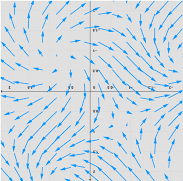
\includegraphics[width=0.4\linewidth]{pic/vector field}

\pp

\bigskip

切空间

\pp
\bigskip

张量场(例如余切向量场(即一阶微分形式),应力张量场等)

\bigskip

\pp

标量场(函数)
\end{frame}



\subsection{严谨定义*}

\subsubsection{严谨定义*}
\begin{frame}\frametitle{严谨定义*}
上述非严谨的定义中,需要固定各线性空间的一组基。而数学和物理中通常希望一个量或者一个概念不依赖于基(坐标系、参考系)的选取。这要求我们内蕴地给出张量积的定义。

\bigskip

在给出严谨定义之前,我们需要引入一些基本概念。
\begin{itemize}
\item 线性函数与对偶空间
\item 多重线性映射(函数)
\end{itemize}
\end{frame}





\subsubsection{Hom空间,线性函数与对偶空间*}
\begin{frame}\frametitle{Hom空间,线性函数与对偶空间*}
设$V$和$W$为有限维$\bF$-线性空间.\pp 从$V$到$W$上的全体线性映射组成的集合记为
\[\blue{\mathrm{Hom}(V,W)} = \{\mA \colon V\rightarrow W\mid \mA \text{为线性映射}\}.\]
\pp
称从$V$到$\bF$的线性映射为$V$上的线性函数.\pp 记
\[\blue{V^*} = \mathrm{Hom}(V,\bF) = \{f\colon V\rightarrow \bF\mid f \text{为线性函数}\}.\]

\pp
\bigskip

在$\mathrm{Hom}(V,W)$以及$V^*$上,按如下方式定义加法和数乘
\begin{equation*}
\begin{split}
& (\blue{f+g})(v) := f(v) + g(v) \\
& (\blue{\lambda f})(v) := \lambda f(v) \\
\end{split}
\end{equation*}
\pp
\begin{proposition}
在上述加法和数乘下, $\mathrm{Hom}(V,W)$ 和 $V^*$均构成$\bF$-线性空间.\pp 称后者为$V$的\blue{对偶空间}.
\end{proposition}
\end{frame}





\subsubsection{对偶空间基本性质*}
\begin{frame}\frametitle{对偶空间基本性质*}

\begin{proposition}[对偶空间的维数与基]
\begin{itemize}
\item 对偶空间$V^*$的维数与$V$的维数相同.\pp
\item 若$e_1,\cdots,e_n$为$V$的一组基,则$V^*$存在唯一的一组基$f_1,\cdots,f_n$满足
\[f_j(e_i)=\delta_{ij}=\left\{{1, \quad \text{若 }i=j;\atop 0,\quad \text{若 }i\neq j}\right..\]\pp
称$f_1,\cdots,f_n$为$e_1,\cdots,e_n$的\blue{对偶基}.
\end{itemize}
\end{proposition}
\pp
我们有如下自然的\blue{取值映射(evaluation map)}:
\[ev\colon V^*\times V\rightarrow \bF; \quad (f,v)\mapsto f(v).\]
\pp
\begin{proposition}
\[ V\cong V^{**} \quad v \mapsto ev(-,v) \]
\end{proposition}
\pp
注: 若我们不要求$V$为有限维的,则映射$V\rightarrow V^{**}$仅为单射.
\end{frame}





\subsubsection{向量的逆变性与对偶向量的协变性*}
\begin{frame}\frametitle{向量的逆变性与对偶向量的协变性*}

\begin{proposition}[向量的逆变性与对偶向量的协变性]
设$e_1,\cdots,e_n$以及 $e'_1,\cdots,e'_n$为$V$为有限维$\bF$-线性空间的两组基.设过渡矩阵为 $A$,即
\[(e'_1,\cdots,e'_n) = (e_1,\cdots,e_n)\blue{A}.\]
记这两组基的对偶基分别为$f_1,\cdots,f_n$和$f'_1,\cdots,f'_n$.
\begin{enumerate}
\item (向量的逆变性) 设$v\in V$在两组基下坐标为$X$和$X'$. 即,
\[v = (e_1,\cdots,e_n)X = (e'_1,\cdots,e'_n)X'.\]
则
\[\blue{X' = A^{-1}X} \quad \text{或} \quad \blue{(x'_1,\cdots,x'_n) = (x_1,\cdots,x_n) (A^{-1})^T}.\]
\item (对偶向量协变性) 设对偶向量$f$在两组对偶基下坐标为$Y$和$Y'$.即,
\[f  = (f_1,\cdots,f_n)Y = (f'_1,\cdots,f'_n)Y'.\]
则
\[\blue{Y' = A^TY}  \quad \text{或} \quad \blue{(y'_1,\cdots,y'_n) = (y_1,\cdots,y_n)A}.\]
\end{enumerate}
\end{proposition}
\yang{证明思路:\[(f'_1,\cdots,f'_n) = (f_1,\cdots,f_n) (A^T)^{-1}.\]}
\end{frame}





\subsubsection{多重线性映射*}
\begin{frame}\frametitle{多重线性映射*}
设 $V_1,V_2,\cdots,V_r,W$为有限维$\bF$-线性空间.\pp 若映射
\[\tau \colon V_1\times V_2\times \cdots \times V_r \rightarrow W\]
对每个分量都是线性的, 即对所有的指标$i=1,2,\cdots,r$,都有
\begin{equation*}
{\small{
\tau(v_1,\cdots,\alpha v_i + \beta v'_i,\cdots,v_r) = \alpha \tau(v_1,\cdots,v_i,\cdots,v_r) + \beta \tau(v_1,\cdots,v'_i,\cdots,v_r),}}
\end{equation*}
则称$\tau$为从$V_1\times V_2\times \cdots \times V_r$到$W$的\blue{多重线性映射}.\pp 特别地,若$W=\bF$,则称多重线性映射
\[\tau \colon V_1\times V_2\times \cdots \times V_r \rightarrow \bF\]
为$V_1\times V_2\times \cdots \times V_r$上的\blue{多重线性函数}.
\end{frame}





\subsubsection{多重线性映射例子*}
\begin{frame}\frametitle{多重线性映射例子*}
\begin{example}[行列式]
行列式$\det \colon \bF^n \times \bF^n \times \cdots \times \bF^n \longrightarrow \bF$为多重线性函数.
\end{example}
\pp
\begin{example}[取值映射]
取值映射$ ev \colon V^*\times V\rightarrow \bF$是双线性函数.
\end{example}

\begin{example}[三维空间的点积]
\[-\cdot- \colon \bR^3\times\bR^3 \rightarrow \bR;\]
\[(a_1,a_2,a_3)\cdot(b_1,b_2,b_3)=a_1b_1+a_2b_2+a_3b_3.\]
\end{example}

\begin{example}[三维空间的叉积]
\[-\times- \colon \bR^3\times\bR^3 \rightarrow \bR^3\]
\[(a_1,a_2,a_3)\times(b_1,b_2,b_3) = (a_2b_3-a_3b_2,a_3b_1-a_1b_3,a_1b_2-a_2b_1).\]
\end{example}

\end{frame}





\subsubsection{多重线性映射组成的空间*}
\begin{frame}\frametitle{多重线性映射组成的空间*}
我们如下定义多重线性映射的加法和数乘.\pp 任取从$V_1\times V_2\times \cdots \times V_r$到$W$的两个多重线性映射$\tau$和$\tau'$,以及$\lambda\in\bF$,
\begin{equation*}
\begin{split}
& (\blue{\tau+\tau'})(v_1,v_2,\cdots,v_n):= \tau(v_1,v_2,\cdots,v_n) + \tau'(v_1,v_2,\cdots,v_n); \\
& (\blue{\lambda\tau})(v_1,v_2,\cdots,v_n):= \lambda\cdot \tau(v_1,v_2,\cdots,v_n).
\end{split}
\end{equation*}
\pp
\begin{proposition}
从$V_1\times V_2\times \cdots \times V_r$到$W$的全体多重线性映射组成的集合在上述加法和数乘下构成$\bF$-线性空间.
\end{proposition}

\end{frame}





\subsubsection{两线性空间的张量积严谨定义*}
\begin{frame}\frametitle{两线性空间的张量积严谨定义*}
设$V$和$W$为两有限维$\bF$-线性空间.
\pp
\begin{definition}[张量积的无坐标化严谨定义]
称线性空间 $\blue{V\otimes W}:=\{\tau \colon V^*\times W^* \rightarrow \bF \mid \tau \text{为双线性函数}\}$
为$V$和$W$的\blue{张量积}.
\end{definition}
\pp
任取$v\in V$以及$w\in W$, 如下定义从$V^*\times W^*$到$\bF$函数
\[(f,g)\mapsto f(v)g(w).\]
则这一函数为双线性的,记为 $\blue{v\otimes w} \in V\otimes W$.
\pp
\begin{proposition}
设$e_1,\cdots,e_m$为$V$的一组基,以及$\eta_1,\cdots,\eta_n$为$W$的一组基.则
\[\{e_i\otimes \eta_j\mid 1\leq i \leq m, 1\leq j \leq n\}\]
为张量积$V\otimes W$的一组基.
\end{proposition}
\pp
\begin{proposition}[张量运算关于分量的线性性]
\[(\alpha v+\beta v')\otimes w =\alpha (v\otimes w) + \beta (v'\otimes w) \in V\otimes W.\]
\[v\otimes(\alpha w+\beta w') =\alpha (v\otimes w) + \beta (v\otimes w') \in V\otimes W.\]
\end{proposition}
\end{frame}

%\subsubsection{什么是向量*}
%\begin{frame}\frametitle{张量积的泛性质(张量积在范畴论中的定义)*}
%\pp
%\begin{proposition}[张量积泛性质]
%\begin{enumerate}
%\item 张量运算 $(v,w)\mapsto v\otimes w$为从$V\times W$到$V\otimes W$的双重线性映射;\pp
%\item 对于任意$\bF$-线性空间$U$,存在如下一一对应
%\[\{f\colon V\times W \rightarrow U \mid f \text{双线性}\} \xleftrightarrow[f=g\circ h]{\quad 1:1 \quad } \{g \colon V\otimes W \rightarrow U\mid g \text{线性}\}\]
%\end{enumerate}
%\end{proposition}
%\end{frame}





\subsubsection{多个线性空间的张量积的严谨定义*}
\begin{frame}\frametitle{多个线性空间的张量积的严谨定义*}
设$V_1,\cdots,V_r$为有限维$\bF$-线性空间.
\pp
\begin{definition}
记$\blue{V_1\otimes \cdots \otimes V_r} :=\{\tau \colon V_1^*\times \cdots \times V_r^* \rightarrow \bF \mid \tau \text{为多重线性函数}\}$. 称这一线性空间为有限维$\bF$-线性空间$V_1,\cdots,V_r$的\blue{张量积},其中的向量均称为\blue{张量}.
\end{definition}
\pp
如下定义$\blue{v_1\otimes \cdots \otimes v_r} \in V_1\otimes \cdots \otimes V_r$:
\[v_1\otimes \cdots \otimes v_r\colon (f_1,\cdots,f_r)\mapsto f_1(v_1)\cdots f_r(v_r).\]
\pp
\begin{proposition}
设$\{e_{ij}\mid j=1,\cdots,n_i\}$为$V_i$的一组基.\pp 则
\[\{e_{1,j_1}\otimes e_{2,j_2} \otimes \cdots \otimes e_{r,j_r} \mid 1\leq i \leq r, 1\leq j_i \leq \dim(V_i)\}\]
为$V_1\otimes \cdots \otimes V_r$的一组基.
\end{proposition}
\end{frame}





\subsubsection{$(p,q)$-型张量*}
\begin{frame}\frametitle{$(p,q)$-型张量*}
设$V$为有限维$\bF$-线性空间.记
\[V^{p,q}:= \underbrace{V\otimes\cdots\otimes V}_{p\text{个}}\otimes\underbrace{V^*\otimes\cdots\otimes V^*}_{q\text{个}}.\]
称向量空间$V^{p,q}$中的向量为$V$上的\blue{$(p,q)$-型张量}.

\begin{lemma}
设$U,V,W$为三个有限维$\bF$-线性空间.则存在如下典范映射
\[ V\cong V\otimes\bF\cong \mathrm{Hom}(\bF,V)\cong \mathrm{Hom}(V^*,\bF),\]
和
\[\mathrm{Hom}(U\otimes V^*,W)\cong\mathrm{Hom}(U,V\otimes W).\]
\end{lemma}

\end{frame}





\subsubsection{$(p,q)$-型张量*}
\begin{frame}\frametitle{$(p,q)$-型张量*}

\begin{theorem}设$V$为有限维$\bF$-线性空间. 则以下三个线性空间之间存在典范同构
\begin{itemize}
\item $\underbrace{V\otimes\cdots\otimes V}_{p\text{个}}\otimes\underbrace{V^*\otimes\cdots\otimes V^*}_{q\text{个}}$
\item $\mathrm{Hom}_{\bF}(\underbrace{V\otimes\cdots\otimes V}_{q\text{个}},\underbrace{V\otimes\cdots\otimes V}_{p\text{个}})$
\item $\mathrm{Hom}_{\bF}\big(\underbrace{V^*\otimes\cdots\otimes V^*}_{p\text{个}}\otimes\underbrace{V\otimes\cdots\otimes V}_{q\text{个}},\bF\big)$
\item 多重线性函数$\phi\colon \underbrace{V^*\times\cdots\times V^*}_{p\text{个}}\times\underbrace{V\times\cdots\times V}_{q\text{个}} \rightarrow \bF$组成的空间.
\end{itemize}
这些空间中的向量都可称为\blue{$(p,q)$-型张量}.
\end{theorem}
\end{frame}





\subsubsection{对称张量积的严谨定义*}
\begin{frame}\frametitle{对称张量积的严谨定义*}
设$V$为有限维$\bF$-线性空间. 设$\tau \colon \underbrace{V^*\times \cdots \times V^*}_{r\text{个}} \rightarrow \bF$为$r$-重线性函数.我们称其为\blue{对称的},若对于任意$1\leq i<j\leq r$以及任意$f_1,f_2,\cdots,f_r\in V^*$, 都有
\[\tau(f_1,\cdots,f_i,\cdots,f_j,\cdots,f_r)=\tau(f_1,\cdots,f_j,\cdots,f_i,\cdots,f_r).\]
\pp
\begin{definition}
记$\blue{\mathrm{Sym}^r(V)} :=\{\tau \colon \underbrace{V^*\times \cdots \times V^*}_{r\text{个}} \rightarrow \bF \mid \tau \text{为对称的$r$重线性函数}\}$. 则这是$V^{\otimes r}$的一个子空间. 称之$V$的\blue{$r$阶对称张量积}.
\end{definition}
\pp
定义
\[v_1\odot v_2\odot \cdots \odot v_r := \frac1{r!}\sum\limits_{\sigma\in S_r} v_{\sigma(1)}\otimes v_{\sigma(2)} \otimes \cdots \otimes v_{\sigma(r)} \in V^{\otimes r}\]
\pp
\begin{proposition}
设$e_1,\cdots,e_n$为$V$的一组基.\pp 则
\[ \{e_{i_1}\odot e_{i_2} \odot \cdots \odot e_{i_r} \mid 1\leq i_1\leq i_2\leq \cdots \leq i_r\leq n\}\]
为$\mathrm{Sym}^r(V)$一组基.
\end{proposition}
\end{frame}





\subsubsection{外积与反对称张量的严谨定义*}
\begin{frame}\frametitle{外积与反对称张量的严谨定义*}
设$V$为有限维$\bF$-线性空间. 设$\tau \colon \underbrace{V^*\times \cdots \times V^*}_{r\text{个}} \rightarrow \bF$为$r$-重线性函数.我们称其为\blue{反对称的},若对于任意$1\leq i<j\leq r$以及任意$f_1,f_2,\cdots,f_r\in V^*$, 都有
\[\tau(f_1,\cdots,f_i,\cdots,f_j,\cdots,f_r)=\blue{-}\tau(f_1,\cdots,f_j,\cdots,f_i,\cdots,f_r).\]
\pp
\begin{definition}
记$\blue{\bigwedge^r(V)} :=\{\tau \colon \underbrace{V^*\times \cdots \times V^*}_{r\text{个}} \rightarrow \bF \mid \tau \text{为反对称的$r$重线性函数}\}$. 则这是$V^{\otimes r}$的一个子空间. 称之$V$的\blue{$r$阶反对称张量积}.
\end{definition}
\pp
定义
\[v_1\wedge v_2\wedge \cdots \wedge v_r := \frac1{r!}\sum\limits_{\sigma\in S_r} (-1)^{\tau(\sigma)} v_{\sigma(1)}\otimes v_{\sigma(2)} \otimes \cdots \otimes v_{\sigma(r)} \in V^{\otimes r}\]
\pp
\begin{proposition}
设$e_1,\cdots,e_n$为$V$的一组基.\pp 则
\[ \{e_{i_1}\wedge e_{i_2} \wedge \cdots \wedge e_{i_r} \mid 1\leq i_1<i_2<\cdots <i_r\leq n\}\]
为$\bigwedge^r(V)$一组基.
\end{proposition}
\end{frame}





\subsubsection{张量的缩并*}
\begin{frame}\frametitle{张量的缩并*}

设$p,q$为正整数.对于任意给定$1\leq i\leq p$和$1\leq j\leq q$,我们有如下缩并映射
\[\Phi^i_j\colon V^{(p,q)} \longrightarrow V^{(p-1,q-1)}\]
其将 $v_1\otimes \cdots \otimes v_i \otimes \cdots \otimes v_p \otimes f_1\otimes \cdots \otimes f_j \otimes \cdots \otimes f_q$映成
\[ f_j(v_i) \cdot (v_1\otimes \cdots \otimes v_{i-1} \otimes v_{i+1} \otimes \cdots \otimes v_p) \otimes (f_1\otimes \cdots \otimes f_{j-1}\otimes f_{j+1}\otimes \cdots \otimes f_q)\]

\begin{proposition}
设$V$和$W$为两有限维$\bF$-线性空间.\pp 则
\begin{enumerate}
\item 存在典范同构
\[W\otimes V^*\cong\mathrm{Hom}(V,W)\]
将$w\otimes f$映成线性映射$(v \mapsto f(v)w)$.
\item 若$W=V$,则上述同构与 $\mathrm{tr}$ (迹) 的合成正好为缩并映射. 即下图交换
\begin{equation*}
\xymatrix{
V\otimes V^* \ar[dr]_{\Phi_1^1} \ar[r]^-{\cong}&  \mathrm{Hom}(V,V) \ar[d]^{\mathrm{tr}}\\
& \bF\\}
\end{equation*}
\end{enumerate}
\end{proposition}
\end{frame}









% ========== 2023年07月04号 第34次课 习题课 ==========








% ========== 2023年07月06号 第35次课 习题课 ==========









